% $Id$
%


%\usebackgroundtemplate{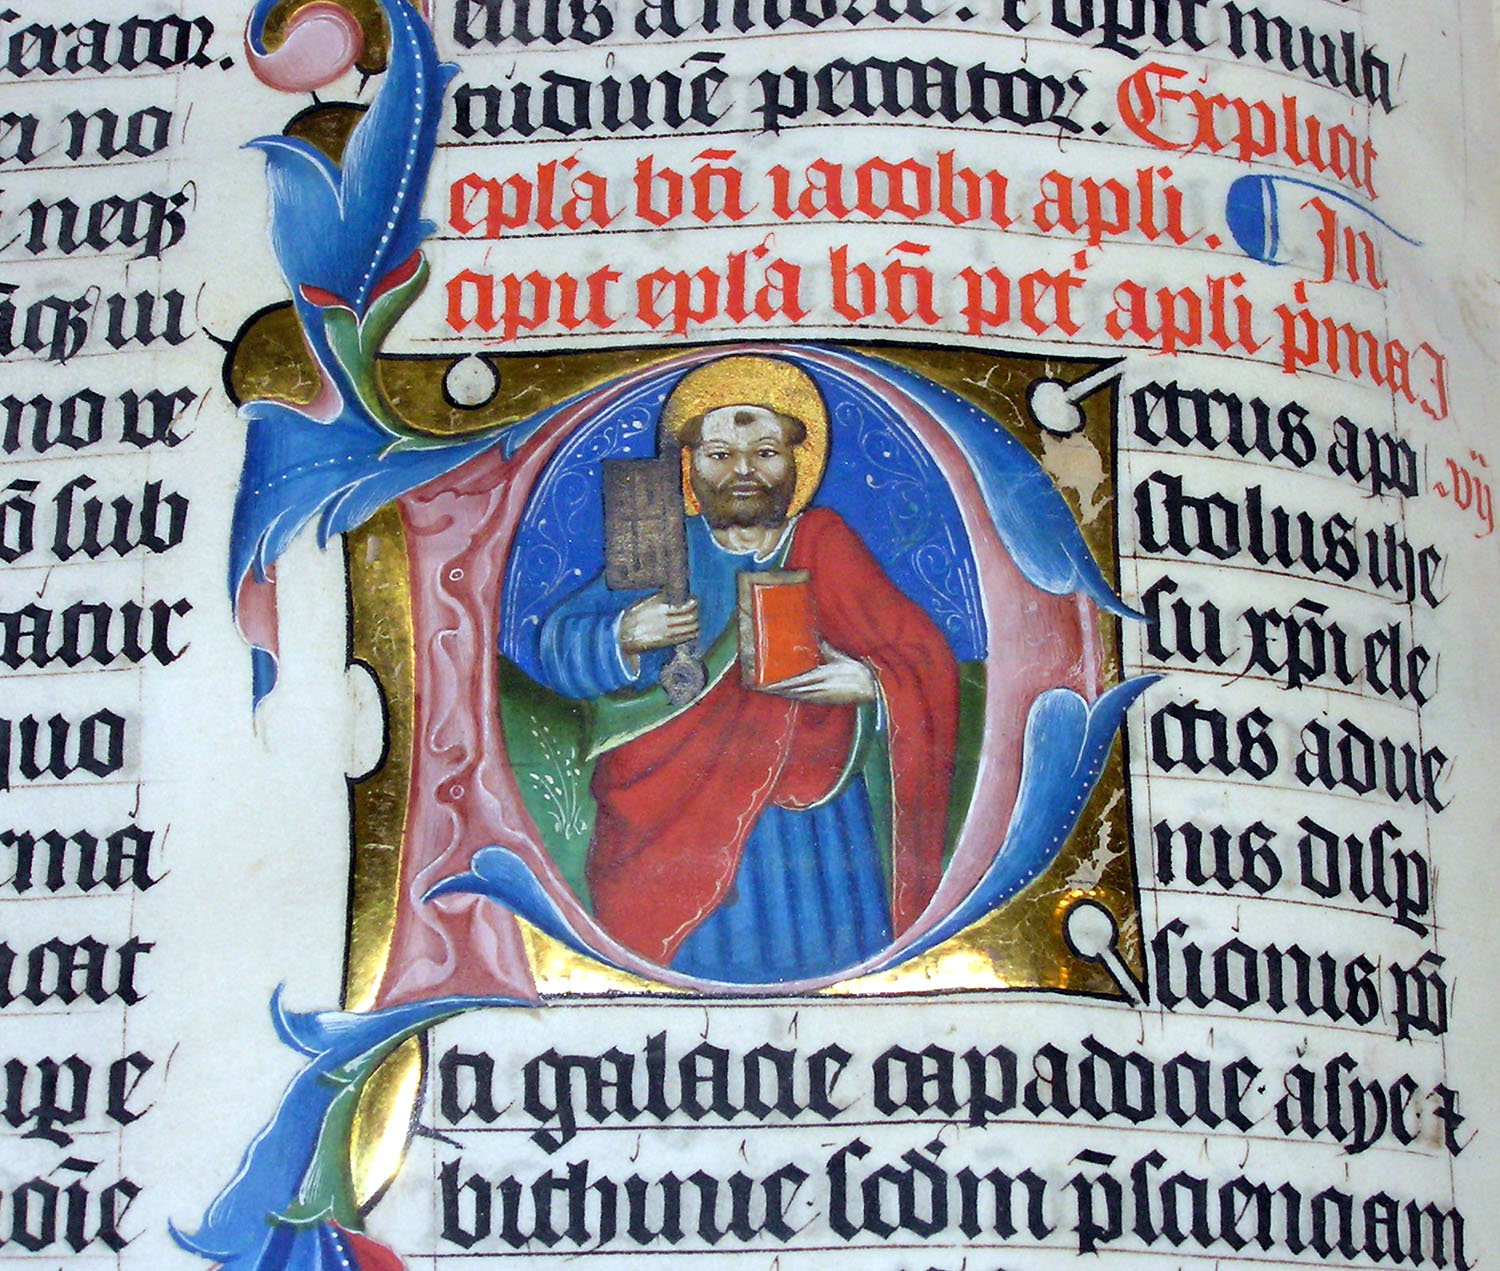
\includegraphics[width=13cm]{figs/biblia}}
%{\bf
%  \textcolor[rgb]{1,1,1}{
    \section{Edici�n en Wikipedia}
%  }
%}

%\usebackgroundtemplate{}

%%---------------------------------------------------------------

\begin{frame}
\frametitle{Colaboraci�n con una comunidad}

{\Large
\begin{itemize}
\item Creaci�n o mejora de art�culos en Wikipedia
\item Muy importante: conocer y respetar las normas de la comunidad
\item Gran impacto fuera del grupo de aprendizaje
\item Incentivo: colaboraci�n en un proyecto muy conocido
\item Atenci�n: Wikipedia es una enciclopedia \\
  �hay que tenerlo en cuenta!
\end{itemize}
}
\end{frame}




